\section{Experimental Setup}

\begin{table*}[!t]
\centering
\setlength{\tabcolsep}{1.5pt}
\resizebox{\textwidth}{!}{%
\begin{tabular}{ll}
    \toprule
    \textbf{Reward type} & \textbf{Formula} \\
    
    \midrule

    Baseline random & \(r(a_t) = \text{Relevance}(d_{a_t, n})\) \text{ where} \(a_t \sim \text{unif}(a_1, ..., a_K), n \sim \text{unif}(rank_1, rank_2, .. rank_m)\) \\[0.5em]
    
    Baseline random rank-aware & \(r(a_t, n) = \text{Relevance}(d_{a_t}, n)\) \text{ where} \(a_t \sim \text{unif}(a_1, ..., a_K)\) \\[0.5em]

    \midrule
    \(\epsilon\)-greedy & \(r(a_t, n) = \text{Relevance}(d_{a_t, n})\) \text{ if} \(\text{Relevance}(d_{a_t, n-1})\) \text{ is 1 else } \(a_t \sim \text{unif}(a_1, ..., a_K)\) \\[0.5em]
    
    Bernoulli & \( r(a_t, n) = \text{Relevance}(d_{a_t, n}) \) \\[0.5em]
    
    Bernoulli UCB & \( r(a_t, n) = \text{Relevance}(d_{a_t, n}) + c \cdot \sqrt{\frac{\log_2(n + 1)}{n}} \quad \text{with } c \to 0 \) \\[0.5em]
    
    Bernoulli top-\(k\) & \( r(a_t, n) = \frac{1}{k} \sum_{i=n}^{n+k-1} \text{Relevance}(d_{a_t, i}) \) \\[0.5em]
    
    Bernoulli rank-aware & \( r(a_t, n) = \frac{\text{Relevance}(d_{a_t, n})}{\log_2(n + 2)} \) \\[0.5em]
    
    Gaussian & \( r(a_t, n) = \text{RFF}(d_{a_t, n}) \quad \text{or} \quad \text{ColBERT}(d_{a_t, n}) \) \\[0.5em]
    
    Diversity & \( r(a_t, n) = \text{Relevance}(d_{a_t, n}) \cdot \left(1 - \frac{\max\limits_{(i, j) \in \mathcal{O}} \cos(d_{a_t, n}, d_{i, j}) + 1}{2}\right) \) \\[0.5em]
    
    Diversity concave & \(
    r(a_t, n) = \text{Relevance}(d_{a_t, n}) \cdot 
    \begin{cases}
    1, & \text{if } \max\limits_{j < n} \cos(d_{a_t, n}, d_{a_t, j}) < 0 \\
    \exp\left(-a \cdot \left(\max\limits_{(i, j) \in \mathcal{O}} \cos(d_{a_t, n}, d_{i, j}))\right)^b\right), & \text{otherwise}
    \end{cases}
    \)  \\[0.5em]

    Bernoulli top-\(k\) UCB diversity & \( r(a_t, n) = \frac{1}{k} \sum_{i=n}^{n+k-1} \text{Relevance}(d_{a_t, i}) \cdot \left(1 - \frac{\max\limits_{(i, j) \in \mathcal{O}} \cos(d_{a_t, n}, d_{i, j})) + 1}{2}\right) + c \cdot \sqrt{\frac{\log_2(n + 1)}{n}}, \text{ with } c \to 0 \)\\
    \bottomrule
    \end{tabular} }
    \caption{Reward policies used for evaluating sub-query selection strategies. For all but the baseline random, we assume \(n = \min \{ j \in \{1,\ldots,N\} \mid (a_t, j) \notin \mathcal{O} \}\). For the diversity concave policy, we assume \(a=5\) and \(b=15\).}
\label{tab:reward_functions}
\end{table*}

We run our experiments on two datasets, which come with different properties and challenges. %: (1) \textbf{NeuCLIR} contains user requests that have to be decomposed and for which we retrieve documents; the sub-queries are generated in a serialized manner, i.e., a one-level decomposition. This dataset is part of TREC for which we have access to nuggets for long-form report generation; (2) \textbf{ResearchyQuestions} contains pre-defined hierarchical sub-queries on two levels, on which we can apply correlated bandits; for this dataset, we do not have a downstream task.

\subsection{NeuCLIR}
\header{Dataset}
The \textbf{NeuCLIR} dataset \cite{lawrie2025overviewtrec2024neuclir} features decomposable user requests; the sub-queries are generated in a serialized manner, i.e., a one-level decomposition. NeuCLIR is part of TREC (Text Retrieval Conference) and is designed to evaluate information retrieval models on multilingual data. More precisely, the dataset contains complex user requests and a corpus of documents in Chinese ($\sim$3M documents), Russian ($\sim$5M documents), and Persian (2M documents). \footnote{\url{https://huggingface.co/neuclir}} For the purpose of this study, all documents have been translated into English. We run our experiments on the entirety of the human-annotated nugget partition of the dataset. The average length of each user request is \(51.95 \pm 19.46\) words.

\header{Retrieval} We decompose NeuCLIR user requests into \(k=16\) sub-queries using LLM calls as specified in prompts \ref{fig:problem-definition-prompt} and \ref{fig:specialized-information-prompt}. For each generated sub-query, we run a search engine to retrieve \(n=10\) documents. The retriever used in this study is a combination of PLAID-X, a dual encoder with late interaction \cite{colbert-x, translate-distill}, learned sparse retrieval (LSR) \cite{LSRandrewThong}, which combines sparse retrieval with contextualized dense embeddings, and a Qwen retriever \cite{bai2023qwentechnicalreport, qwen2025qwen25technicalreport}.

\begin{figure*}[t!]
    \centering
    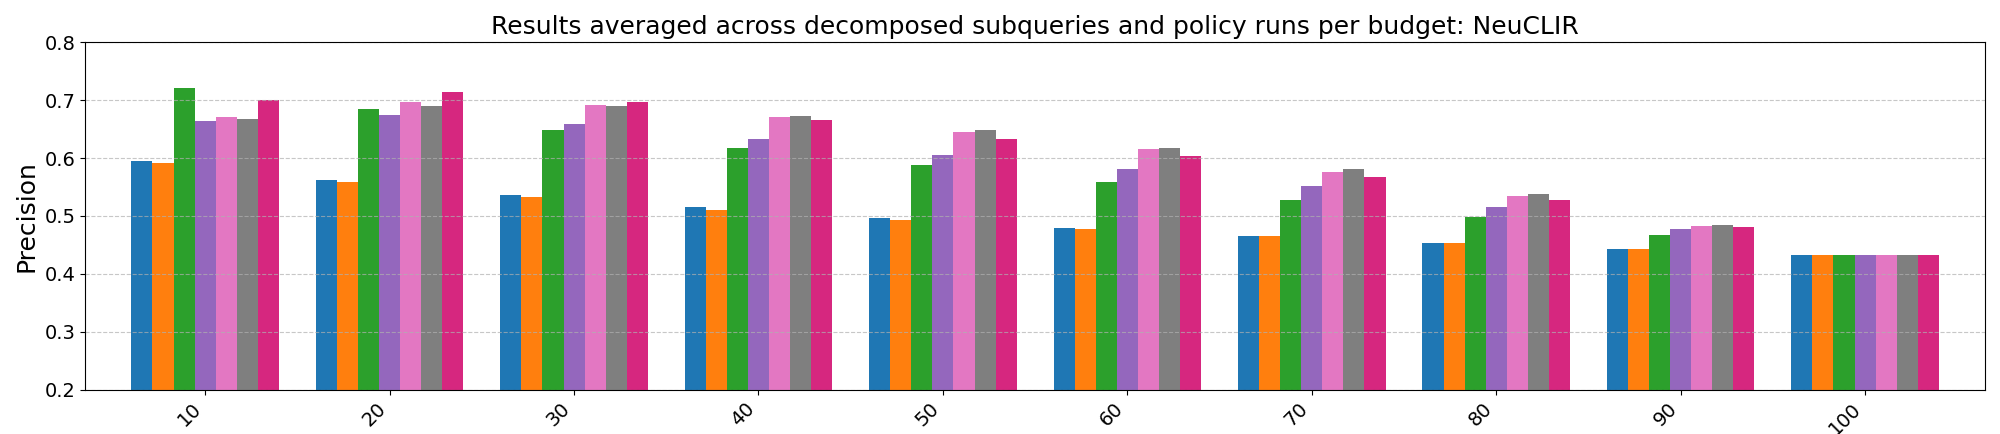
\includegraphics[width=\linewidth]{images/NeuCLIR/precision_few_small_axis_cropped.png}
    \vspace{1em}  % optional spacing between figures
    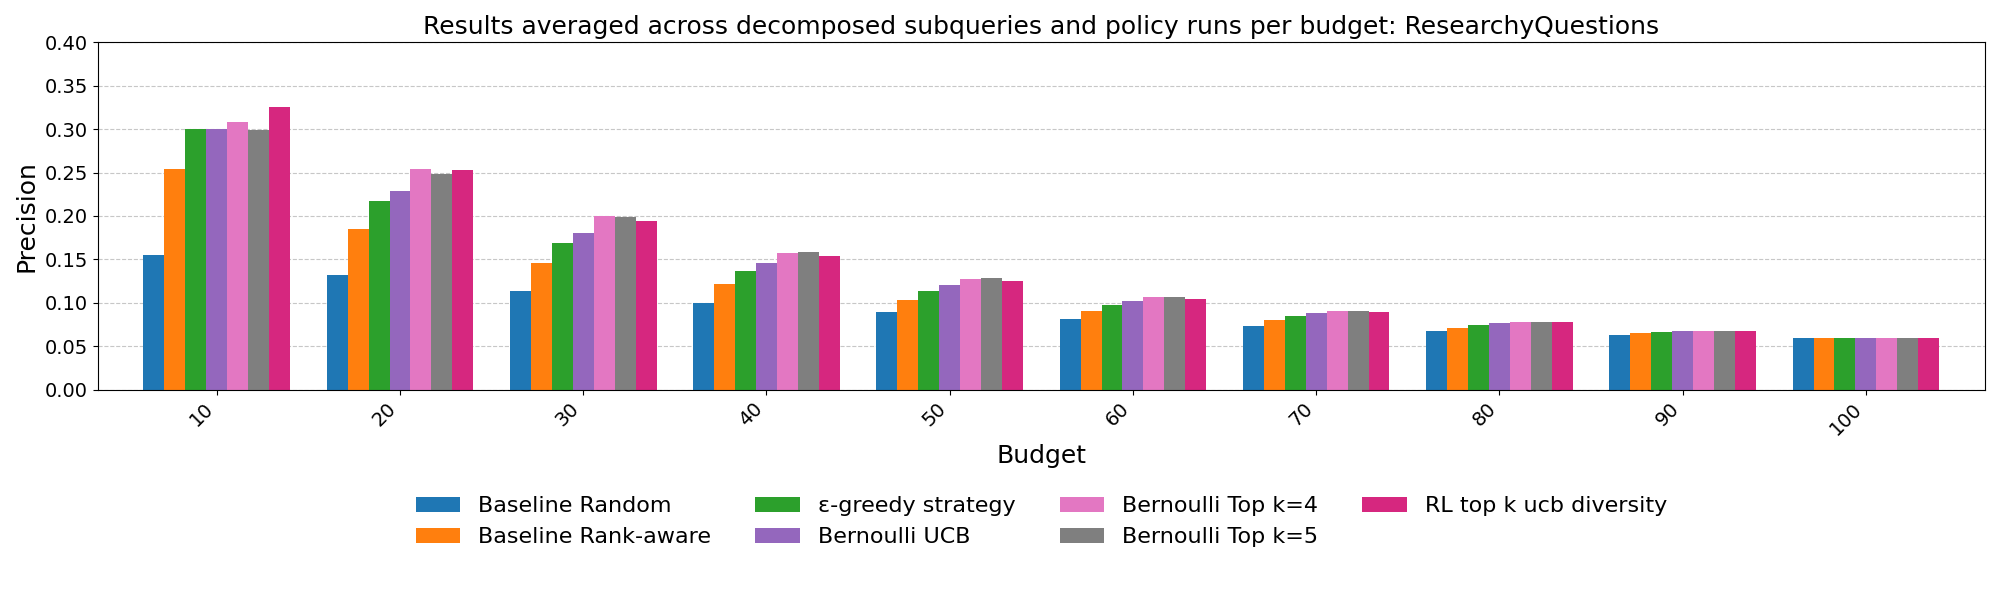
\includegraphics[width=\linewidth]{images/Researchy/precision_few_small_axis.png}
    \vspace*{-13mm}
    \caption{Precision scores on NeuCLIR24 and ResearchyQuestions for baselines and reward policies, evaluated across varying budgets of observed documents. The budgets are expressed as percentages of the total available corpus. Modelling the queries using Bernoulli distribution considering the top ranked k documents performs the best across budgets, with all policies reaching the same performance as the budget covers the whole space of actions.}
    \label{fig:neuclir_precision}
\end{figure*}



\subsection{ResearchyQuestions}
\textbf{Dataset.} 
ResearchyQuestions \cite{rosset2024researchyquestionsdatasetmultiperspective} is composed of \(100k\) complex Bing questions that are non-factoid, multi-perspective, and require decomposition. Each instance in the dataset is decomposed into sub-queries hierarchically over two levels: %, i.e., some sub-queries are further decomposed into more fine-grained sub-queries. Each instance in the dataset contains a user query that is hierarchically decomposed into two levels: 
\textit{headers} (first-level sub-queries), and \textit{sub-queries} (second-level). We build the corpus by aggregating all documents marked as relevant across the entire ResearchyQuestions dataset. 

\header{Retrieval} We apply BM25 to retrieve top 10 documents for each query. Since some instances have limited document coverage, we filter the data and keep only those where at least 10\% of the retrieved documents are labeled as relevant. The final dataset used for evaluation consists of 140 instances.



% \begin{figure*}[t!]
%     \centering
%     \includegraphics[width=\linewidth]{images/NeuCLIR/recall_few_big_axis_cropped.png}
%     \vspace{1em}  % optional spacing between figures
%     \includegraphics[width=\linewidth]{images/Researchy/recall_few_small_axis.png}
%     \vspace*{-13mm}    
%     \caption{Recall performance of baselines and reward policies under different budget constraints for observed documents. Bernoulli models that take into account information from the top-k ranked documents consistently yield highest recall.}
%     \label{fig:neuclir_recall}
% \end{figure*}

\subsection{Implementation Details}

\header{Rewards} We experiment with the reward introduced in Equation \ref{eq:top_reward} and with several alternatives and baselines described in Table \ref{tab:reward_functions}. We sample documents up to a budget \( b \in \{10\%, 20\%, \ldots, 100\%\} \) out of the total document set of size \(N \times K\). For \(b = 100\%\) we expect all policies and baselines to converge to the same performance. To eliminate noise from random policy starts, we run each experiment \(1000\) times. Moreover, as we decompose the user request using LLM calls, we run the decomposition \(10\) times for each user request, leading to a total of $19 \times 10 \times 1000$ experiments over which we average for each budget. For the Gaussian reward, we experiment with both the RFF and PLAID-X ranking scores, depending on the search engine used. For the diversity concave reward, we set hyperparameters \(a = 5\) and \(b = 15\). 
%For correlated bandits, we verity the utility of a parents sub-query when it has been observed 3 times, we set relevance treshold \(\tau>0.3\) and information transfer hyperparameter \(\lambda=1\).

\header{Metrics} We evaluate performance using precision and \(\alpha\)-nDCG \cite{alphandcg} for document selection. %For \(\alpha\)-nDCG, because of averaging over different runs with potentially different length sets of documents (multiple arms can have overlap in documents, therefore when evaluating the performance of the selected documents, we have to take the set which may vary in length each time), we calculate the minimum set length over all experiments under one budget and use that as our value of k. 
For long-form report generation, we use the Auto-ARGUE framework \cite{autoargue}.

